%\VignetteIndexEntry{The qsmooth user's guide}
%\VignettePackage{qsmooth}
%\VignetteEngine{knitr::knitr}
\documentclass{article}\usepackage[]{graphicx}\usepackage[usenames,dvipsnames]{color}
%% maxwidth is the original width if it is less than linewidth
%% otherwise use linewidth (to make sure the graphics do not exceed the margin)
\makeatletter
\def\maxwidth{ %
  \ifdim\Gin@nat@width>\linewidth
    \linewidth
  \else
    \Gin@nat@width
  \fi
}
\makeatother

\definecolor{fgcolor}{rgb}{0.345, 0.345, 0.345}
\newcommand{\hlnum}[1]{\textcolor[rgb]{0.686,0.059,0.569}{#1}}%
\newcommand{\hlstr}[1]{\textcolor[rgb]{0.192,0.494,0.8}{#1}}%
\newcommand{\hlcom}[1]{\textcolor[rgb]{0.678,0.584,0.686}{\textit{#1}}}%
\newcommand{\hlopt}[1]{\textcolor[rgb]{0,0,0}{#1}}%
\newcommand{\hlstd}[1]{\textcolor[rgb]{0.345,0.345,0.345}{#1}}%
\newcommand{\hlkwa}[1]{\textcolor[rgb]{0.161,0.373,0.58}{\textbf{#1}}}%
\newcommand{\hlkwb}[1]{\textcolor[rgb]{0.69,0.353,0.396}{#1}}%
\newcommand{\hlkwc}[1]{\textcolor[rgb]{0.333,0.667,0.333}{#1}}%
\newcommand{\hlkwd}[1]{\textcolor[rgb]{0.737,0.353,0.396}{\textbf{#1}}}%

\usepackage{framed}
\makeatletter
\newenvironment{kframe}{%
 \def\at@end@of@kframe{}%
 \ifinner\ifhmode%
  \def\at@end@of@kframe{\end{minipage}}%
  \begin{minipage}{\columnwidth}%
 \fi\fi%
 \def\FrameCommand##1{\hskip\@totalleftmargin \hskip-\fboxsep
 \colorbox{shadecolor}{##1}\hskip-\fboxsep
     % There is no \\@totalrightmargin, so:
     \hskip-\linewidth \hskip-\@totalleftmargin \hskip\columnwidth}%
 \MakeFramed {\advance\hsize-\width
   \@totalleftmargin\z@ \linewidth\hsize
   \@setminipage}}%
 {\par\unskip\endMakeFramed%
 \at@end@of@kframe}
\makeatother

\definecolor{shadecolor}{rgb}{.97, .97, .97}
\definecolor{messagecolor}{rgb}{0, 0, 0}
\definecolor{warningcolor}{rgb}{1, 0, 1}
\definecolor{errorcolor}{rgb}{1, 0, 0}
\newenvironment{knitrout}{}{} % an empty environment to be redefined in TeX

\usepackage{alltt}

\RequirePackage{/Library/Frameworks/R.framework/Versions/3.2/Resources/library/BiocStyle/resources/latex/Bioconductor}

\AtBeginDocument{\bibliographystyle{/Library/Frameworks/R.framework/Versions/3.2/Resources/library/BiocStyle/resources/latex/unsrturl}}


\setlength{\parskip}{1\baselineskip}
\setlength{\parindent}{0pt}

\title{The \texttt{qsmooth} user's guide}
\author{Kwame Okrah \texttt{okrah.kwame@gene.com} \and
Hector Corrado Bravo \texttt{hcorrada@gmail.com} \and
Stephanie C. Hicks \texttt{shicks@jimmy.harvard.edu} \and
Rafael A. Irizarry \texttt{rafa@jimmy.harvard.edu} }

\date{Modified: March 5, 2015.  Compiled: \today}
\IfFileExists{upquote.sty}{\usepackage{upquote}}{}
\begin{document}

\maketitle
 
\tableofcontents

\section{Introduction}

In the advent of high-throughput technologies
(such as microarray and RNA-seq) crude assumptions 
were made in order to pre-process and normalize 
the data \cite{loven2012revisiting}.
These crude assumptions were needed because
of large technical variablilty and very few samples
sizes. 
For some data sets the normalization techniques 
based on these crude assumptions lead to a 
significant loss in biological information
\cite{loven2012revisiting, hicks}.
With the current improvements in technology and 
reduction in cost we are now able to relax some
of the previous assumptions to allow for a more
nuanced and information retaining normalization 
techniques.
In this vignette we introduce,
smooth quantile normalization (\texttt{\bf{qsmooth}}), 
a generalization of quantile normalization \cite{bolstad2003comparison}
that makes the assumption that: all samples within the same biological 
group should have the same shape.

\texttt{\bf{Qsmooth}} first performs quantile normalization within 
each biological group and then shrinks the group quantiles
towards the overall reference quantile depending on the variation 
between the group quantiles and the variation of quantiles 
within the groups. The alogorithm is described in Figure \ref{algo}
below. Let gene$(g)$ denote the g${}^{th}$ row after sorting each 
column in the data. 
For each row gene$(g)$ we compute the weight $w_{(g)} \in [0, 1]$.
Where a 0 weight implies quantile normalization within groups and
a weight of 1 indicates quantile normalization across the groups.
The weight at each row depends on the between group sum of squares
$(SSB_{(g)})$ and total sum of squares 
$(SST_{(g)})$, as follow median$\{1 - SSB_{(g)} / SST_{(g)} | g = g -k, g, g+k \}$,
where $k=$floor(total number of genes* 0.05).

\begin{figure}[!h]
\begin{center}
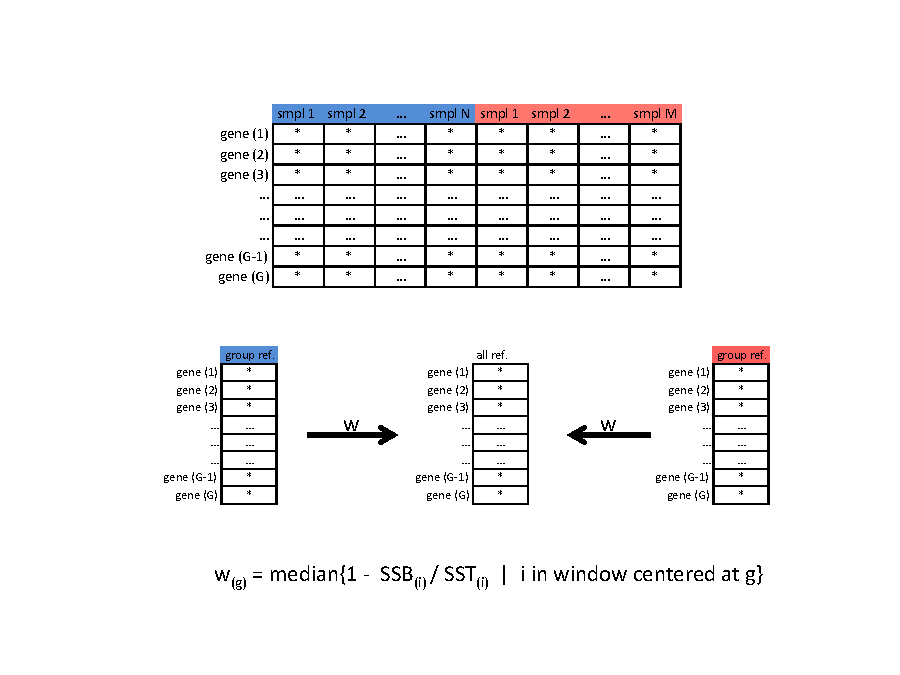
\includegraphics[width=\columnwidth]{qsmooth_algo.pdf}
\end{center}
\small\normalsize
\caption[qsmooth algorithm]
         {{\bf The qsmooth algorithm.} 
          At each quantile compute $R^2$.}
\label{algo}
\end{figure}

\newpage
\section{Rat bodymap}

\subsection{Data 1}

We begin by loading the \texttt{\bf{qsmooth}} into R. 

\begin{knitrout}
\definecolor{shadecolor}{rgb}{0.969, 0.969, 0.969}\color{fgcolor}\begin{kframe}
\begin{alltt}
\hlkwd{library}\hlstd{(qsmooth)}
\end{alltt}
\end{kframe}
\end{knitrout}

The first example is based a data set (data1)
which contains lung samples from 21 week old male and female rats. 
Four samples are from males and four samples are from females.



Below are the boxplots and the density estimate plots
of the raw counts after after adding 1 and 
followed by a log2 transformation (ie. log2(counts+1)).

\begin{knitrout}
\definecolor{shadecolor}{rgb}{0.969, 0.969, 0.969}\color{fgcolor}

{\centering 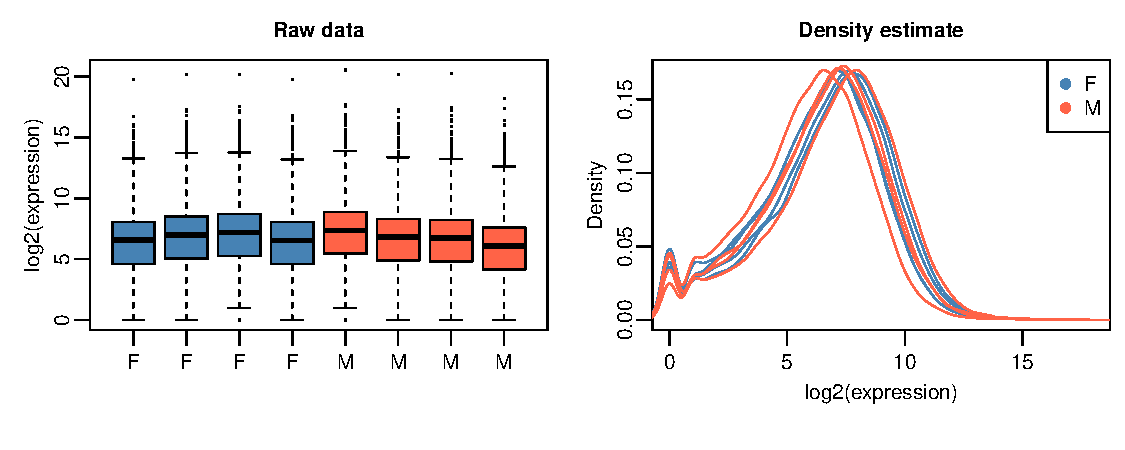
\includegraphics[width=\maxwidth]{figure/raw1-1} 

}



\end{knitrout}

To run the \texttt{\bf{qsmooth}} algorithm on the log transformed raw counts.
We must specify sample groups. 
In this example we will use sex as the grouping factor.

\begin{knitrout}
\definecolor{shadecolor}{rgb}{0.969, 0.969, 0.969}\color{fgcolor}\begin{kframe}
\begin{alltt}
\hlstd{norm.data1} \hlkwb{=} \hlkwd{qsmooth}\hlstd{(}\hlkwc{exprs}\hlstd{=data1,} \hlkwc{groups}\hlstd{=sex,} \hlkwc{plot}\hlstd{=}\hlnum{TRUE}\hlstd{)}
\end{alltt}
\end{kframe}

{\centering 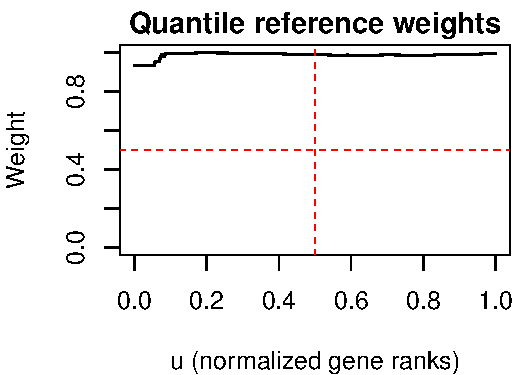
\includegraphics[width=\maxwidth]{figure/qsmooth1-1} 

}



\end{knitrout}

The parameter plot=TRUE indicates that we want to see the 
weigths of interpolation.
Weights are computed for each quantile in the data set.
A weight of 1 indicates full quantile normalization,
where as a weight of 0 indicates quantile normalization
within the groups.

In this example the weights are mostly close to 1,
indicating that the is no major difference between the 
quantiles from the female and male samples.
Here the \texttt{\bf{qsmooth}} algorithm outputs results
that is identical (for practical purposes)
to full quantile normalization. 

\begin{knitrout}
\definecolor{shadecolor}{rgb}{0.969, 0.969, 0.969}\color{fgcolor}

{\centering 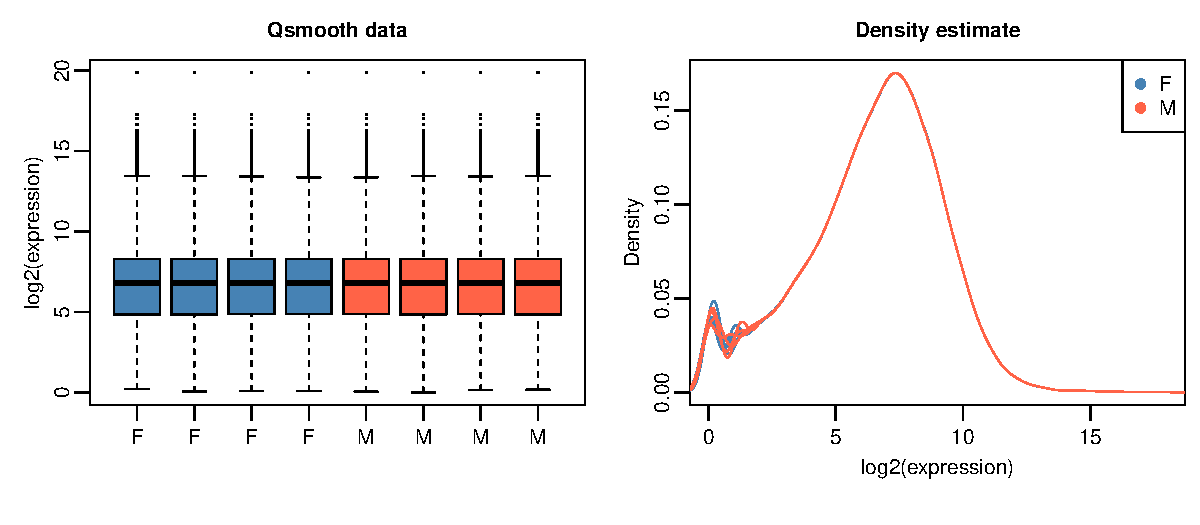
\includegraphics[width=\maxwidth]{figure/norm_data1-1} 

}



\end{knitrout}

\subsection{Example 2}
The first examples consists of a data set which contains lung samples 
from 21 week old male and female rats. 
Four samples from males and a four samples from females.



Let's take a look at the raw data. 
Below is the boxplot and the density plot
of the raw counts after after adding 1 followed by a 
log2 transformation.

\begin{knitrout}
\definecolor{shadecolor}{rgb}{0.969, 0.969, 0.969}\color{fgcolor}

{\centering 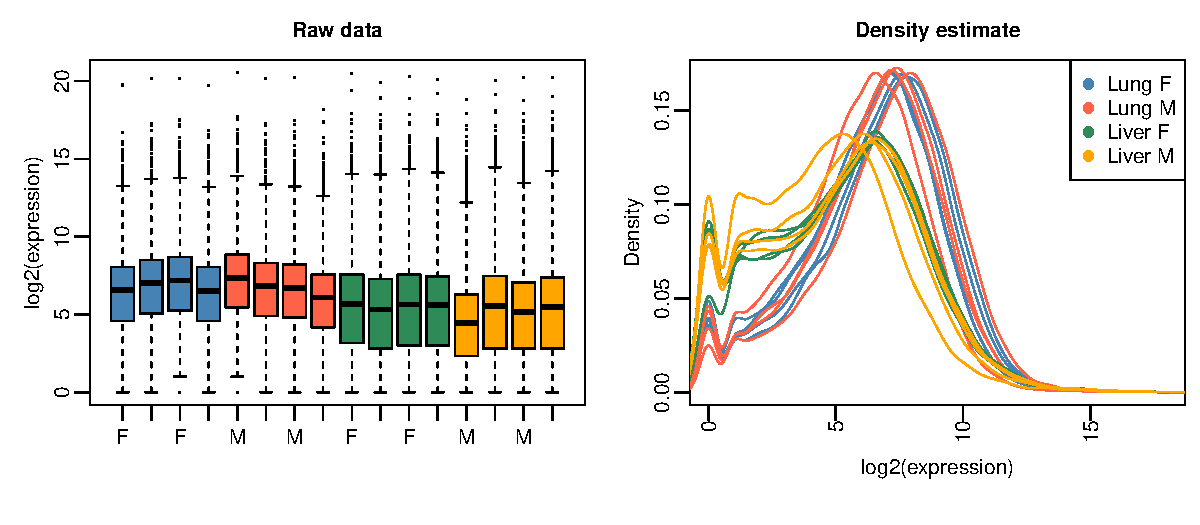
\includegraphics[width=\maxwidth]{figure/raw12-1} 

}



\end{knitrout}

We now run the qsmooth algorithm on the log transform raw counts.
First we must specify sample groups. In this example we specify
the groupings using sex 
\begin{knitrout}
\definecolor{shadecolor}{rgb}{0.969, 0.969, 0.969}\color{fgcolor}\begin{kframe}
\begin{alltt}
\hlstd{norm.data2} \hlkwb{=} \hlkwd{qsmooth}\hlstd{(}\hlkwc{exprs}\hlstd{=data2,} \hlkwc{groups}\hlstd{=}\hlkwd{paste0}\hlstd{(sex, organ),} \hlkwc{plot}\hlstd{=}\hlnum{TRUE}\hlstd{)}
\end{alltt}
\end{kframe}

{\centering 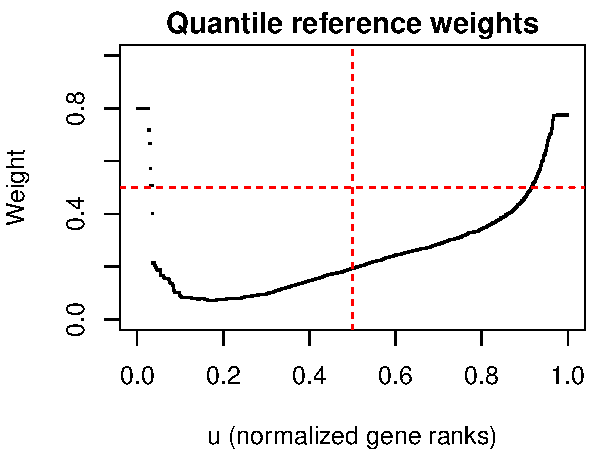
\includegraphics[width=\maxwidth]{figure/qsmooth12-1} 

}



\end{knitrout}

\begin{knitrout}
\definecolor{shadecolor}{rgb}{0.969, 0.969, 0.969}\color{fgcolor}

{\centering 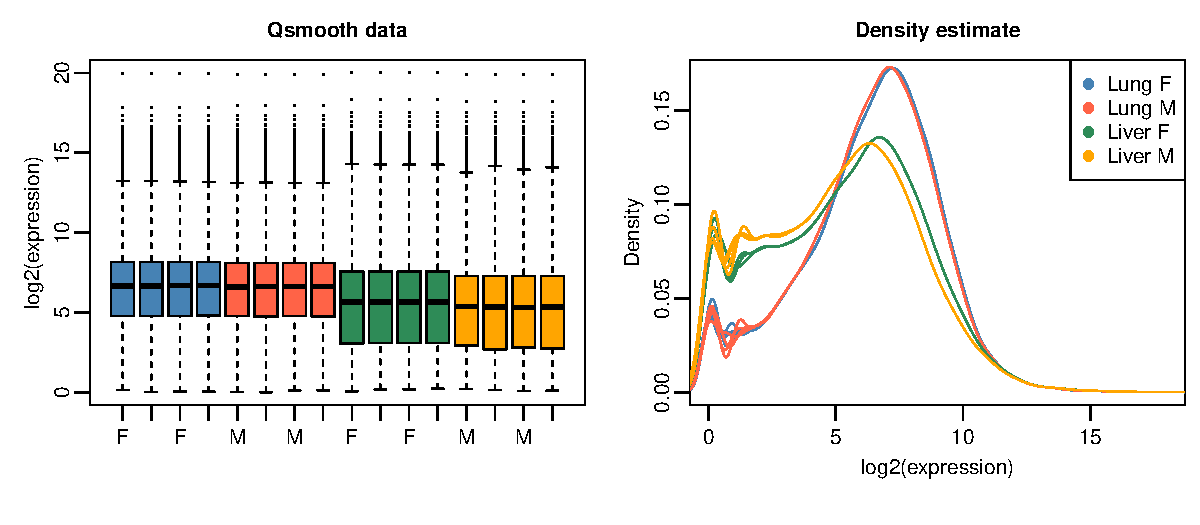
\includegraphics[width=\maxwidth]{figure/norm_data12-1} 

}



\end{knitrout}

\section{Qsmooth}
The \texttt{qsmooth} function accepts four parameters. 
Two are required and the other two are optional.
The \texttt{qsmooth} function requires an expression matrix and a 
character vector or factor specifying which group a sample belongs,
for the exprs and groups parameters respectively.
The \texttt{plot} parameter is optional. It specifies whether or
not the weights should be plotted. It is set to FALSE be defualt.
The \texttt{norm.factors} allows the user to specify a 
vector of scaling factors that will be used to modify the 
expression data set prior to applying the qsmooth algorithm.

\subsection{Pre-specified scaling factors}

\begin{knitrout}
\definecolor{shadecolor}{rgb}{0.969, 0.969, 0.969}\color{fgcolor}\begin{kframe}
\begin{alltt}
\hlstd{norm.data3} \hlkwb{=} \hlkwd{qsmooth}\hlstd{(}\hlkwc{exprs}\hlstd{=data2,} \hlkwc{groups}\hlstd{=}\hlkwd{paste0}\hlstd{(sex, organ),}
                     \hlkwc{norm.factors} \hlstd{=} \hlkwd{apply}\hlstd{(data2,} \hlnum{2}\hlstd{, mean))}
\end{alltt}
\end{kframe}
\end{knitrout}

\begin{knitrout}
\definecolor{shadecolor}{rgb}{0.969, 0.969, 0.969}\color{fgcolor}\begin{kframe}
\begin{alltt}
\hlkwd{par}\hlstd{(}\hlkwc{mar}\hlstd{=}\hlkwd{c}\hlstd{(}\hlnum{4}\hlstd{,} \hlnum{3}\hlstd{,} \hlnum{2}\hlstd{,} \hlnum{0.5}\hlstd{),} \hlkwc{mgp}\hlstd{=}\hlkwd{c}\hlstd{(}\hlnum{1.5}\hlstd{,} \hlnum{0.5}\hlstd{,} \hlnum{0}\hlstd{),} \hlkwc{cex.axis}\hlstd{=}\hlnum{0.8}\hlstd{,} \hlkwc{cex.lab}\hlstd{=}\hlnum{0.8}\hlstd{,} \hlkwc{cex.main}\hlstd{=}\hlnum{0.8}\hlstd{)}

\hlcom{# boxplot}
\hlkwd{boxplot}\hlstd{(norm.data3,} \hlkwc{col}\hlstd{=col,} \hlkwc{main}\hlstd{=}\hlstr{"Qsmooth data"}\hlstd{,}
        \hlkwc{names}\hlstd{=sex,} \hlkwc{ylab}\hlstd{=}\hlstr{"log2(expression)"}\hlstd{,} \hlkwc{pch}\hlstd{=}\hlstr{"."}\hlstd{,}
        \hlkwc{cex.axis}\hlstd{=}\hlnum{0.8}\hlstd{)}
\end{alltt}
\end{kframe}

{\centering 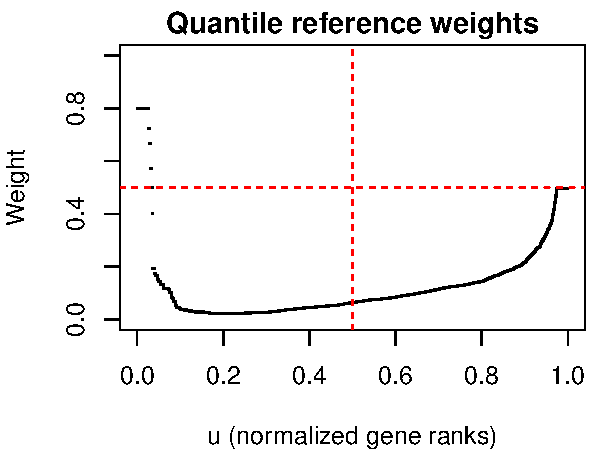
\includegraphics[width=\maxwidth]{figure/qsmooth14-1} 

}



\end{knitrout}

\section{SessionInfo}

\begin{knitrout}
\definecolor{shadecolor}{rgb}{0.969, 0.969, 0.969}\color{fgcolor}\begin{kframe}
\begin{alltt}
\hlkwd{sessionInfo}\hlstd{()}
\end{alltt}
\begin{verbatim}
## R version 3.2.1 (2015-06-18)
## Platform: x86_64-apple-darwin13.4.0 (64-bit)
## Running under: OS X 10.10.5 (Yosemite)
## 
## locale:
## [1] en_US.UTF-8/en_US.UTF-8/en_US.UTF-8/C/en_US.UTF-8/en_US.UTF-8
## 
## attached base packages:
## [1] parallel  stats     graphics  grDevices utils     datasets  methods   base     
## 
## other attached packages:
## [1] bodymapRat_0.0.1    Biobase_2.28.0      BiocGenerics_0.14.0 qsmooth_0.0.0.9000 
## [5] knitr_1.11         
## 
## loaded via a namespace (and not attached):
## [1] BiocStyle_1.6.0 magrittr_1.5    formatR_1.2.1   tools_3.2.1     stringi_1.0-1  
## [6] highr_0.5.1     stringr_1.0.0   evaluate_0.8
\end{verbatim}
\end{kframe}
\end{knitrout}

\bibliography{myrefs}

\end{document}
